% !TeX program = lualatex
% !BIB program = biber
% Projeto UnDF-TeX. LPPL 1.3c ou posterior.
% Exemplo preenchido de entrega institucional, com pessoas fictícias.
\documentclass[perfil=artigo]{undftex}
\usepackage{tikz}
\usepackage{array}
% Mesma composição das referências do artigo autônomo preenchido.
\setcounter{biburllcpenalty}{100}
\setcounter{biburlucpenalty}{200}
\setcounter{biburlnumpenalty}{100}

% !TeX root = ../../artigo-exemplo-undf.tex
\autor{Autoria demonstrativa do UnDF-TeX}
\titulo{Consistência estrutural de documentos acadêmicos em LaTeX}
\subtitulo{estudo didático de verificação do UnDF-TeX}
\identificacaoautor{Autoria ilustrativa, sem atribuição a estudante ou pesquisador real.}
\vinculoautor{Material de demonstração do projeto UnDF-TeX.}
\emailautor{exemplo@example.org}

\curso{Ciência da Computação}
\tipotrabalho{Trabalho de Conclusão de Curso em formato de artigo}
\graupretendido{bacharel em Ciência da Computação}
\objetivo{Exemplo didático de Trabalho de Conclusão de Curso em formato de artigo
para o curso de Ciência da Computação da UnDF. Documento demonstrativo, sem
submissão ou aprovação acadêmica.}
\local{Brasília}
\ano{2026}
\orientador{Ana Exemplo (nome fictício)}
\dataaprovacao{Folha demonstrativa: não houve defesa ou aprovação.}
\limparmembrosbanca
\membrobanca{Ana Exemplo (nome fictício)}{Profa. Dra.}{UnDF -- vínculo ilustrativo}
\membrobanca{Bruno Exemplo (nome fictício)}{Prof. Dr.}{UnDF -- vínculo ilustrativo}
\membrobanca{Carla Exemplo (nome fictício)}{Profa. Dra.}{UnDF -- vínculo ilustrativo}
\addbibresource{exemplo/artigo/referencias.bib}

\undfresetpretextualcontents
% !TeX root = ../../artigo-exemplo-undf.tex
\undfsetcontent{resumo}{%
A reutilização de uma classe LaTeX em diferentes modalidades de trabalho
acadêmico exige verificar numeração, bibliografia e continuidade do texto.
Este estudo didático tem como objetivo examinar a consistência estrutural dos
perfis de monografia e artigo do UnDF-TeX. O procedimento consiste na análise
de casos mínimos com dados sintéticos, compilação por LuaLaTeX e Biber,
extração de texto e inspeção dos documentos produzidos. O corpus compreende
quatro modelos principais e casos específicos de complementos, citação de
citação, objetos extensos e inclusão de PDF. Na revisão local de 14 de outubro
de 2026, os 48 destinos de referências cruzadas dos complementos corresponderam
às páginas registradas nos arquivos auxiliares. Os quatro cenários de citação
de citação produziram as listas bibliográficas previstas, e os testes de
objetos extensos e inclusão de PDF passaram. Os resultados sustentam a
consistência dos comportamentos examinados na versão observada. Não permitem
concluir conformidade normativa integral, aprovação institucional ou ausência
de defeitos em documentos arbitrários. Conclui-se que casos mínimos e revisão
visual oferecem evidências complementares para a manutenção do modelo.}
\undfsetcontent{palavraschave}{documentos acadêmicos; LaTeX; testes de regressão; referências cruzadas}


\begin{document}
  % Mantenha somente os elementos institucionais exigidos pelo curso.
  \undfcover
  \pretextual
  \undffolhaderosto
  \undffolhadeaprovacao

  % O único resumo é impresso na abertura do artigo.
  \undfinicioartigo
  % !TeX root = ../../artigo-exemplo-undf.tex
% Relato didático apoiado em evidências locais; não inventa coleta com participantes.
\section{Introdução}

Uma classe de documentos acadêmicos reúne decisões de apresentação que se
repetem ao longo de um trabalho: títulos, numeração, legendas, citações e
referências. Quando a mesma implementação passa a atender monografias e
artigos, alterações em um mecanismo compartilhado podem afetar documentos
com estruturas distintas. A compilação sem erro é necessária, mas não informa,
por si só, se uma referência conduz à página correta ou se uma obra foi
incluída indevidamente na bibliografia.

O UnDF-TeX oferece um contexto delimitado para examinar esse problema. Seu
perfil de artigo utiliza seções contínuas e não gera automaticamente a
apresentação pré-textual da monografia. Ambos compartilham recursos de
citações e referências cruzadas. A questão deste estudo é: os casos mínimos
da revisão estrutural produzem a numeração, os destinos e as listas
bibliográficas previstos nos dois perfis?

O objetivo é analisar as evidências de consistência registradas nessa revisão
e explicitar o alcance de cada verificação. Trata-se de um exemplo preenchido
de artigo, com autoria demonstrativa e dados de teste. O relato se apoia no
registro técnico do próprio projeto \citeind{undf-verificacao}; não apresenta
pesquisa com participantes nem atribui aprovação acadêmica ao modelo.

\section{Fundamentação e delimitação}

O LaTeX separa a descrição do conteúdo de decisões de composição definidas na
classe e nos pacotes. Entre suas funcionalidades estão referências cruzadas,
fórmulas matemáticas e bibliografias \citeind{latex-introducao}. Essa separação
permite reutilizar uma estrutura documental, mas também concentra
responsabilidades: um erro no tratamento de contadores pode aparecer em
todos os trabalhos que utilizem o mesmo comando.

A bibliografia acrescenta uma etapa de processamento. O BibLaTeX organiza
citações e listas bibliográficas, utiliza Biber como processador de dados e
oferece recursos de filtragem e subdivisão da bibliografia
\citeind{ctan-biblatex}. No UnDF-TeX, uma camada própria distingue a consulta
independente de uma obra de seu uso apenas como fonte original em uma citação
de citação. Por isso, conferir somente a presença da chamada no texto seria
insuficiente para avaliar esse comportamento.

Neste estudo, consistência estrutural significa a correspondência entre
resultados esperados, definidos nos casos de teste, e resultados observados
nos arquivos produzidos. Essa definição não equivale a conformidade integral
com normas de documentação. A pertinência das seções, a qualidade da pesquisa
e as exigências do curso dependem de avaliação que ultrapassa o escopo dos
testes descritos.

\section{Procedimentos de verificação}

\subsection{Corpus e condições de observação}

Foi analisada a revisão local de 14 de outubro de 2026, registrada no commit
\texttt{242953c} da branch \texttt{feature/perfis-tcc}. O corpus reúne os quatro
modelos então existentes: monografia em branco, monografia preenchida,
artigo autônomo e entrega institucional demonstrativa do artigo. Acrescentam-se
casos mínimos para complementos nos dois perfis, quatro cenários de citação
de citação, objetos extensos e inclusão de um PDF externo. Este artigo
preenchido foi criado depois dessa revisão e não integra a contagem dos
quatro modelos observados.

Os dados dos testes são sintéticos. Os nomes de autores usados nos casos de
citação de citação não representam obras consultadas para este artigo. Os
procedimentos consistiram em compilar os documentos com LuaLaTeX, processar
a bibliografia com Biber, recompilar para estabilizar as referências e
examinar os resultados. O registro técnico permite localizar os arquivos de
teste e reproduzir a sequência \citeind{undf-verificacao}.

\subsection{Critérios e sequência de análise}

Foram adotados três tipos de evidência: asserções de contadores durante a
compilação, leitura dos arquivos auxiliares e do texto extraído, e inspeção
do PDF. A \figuraref{verificacao} representa a sequência de análise. As etapas
se complementam: a leitura de texto pode localizar uma legenda, enquanto a
inspeção visual permite avaliar seu encaixe na página.

\begin{figure}[htb]
  \centering
  \caption{Sequência de verificação dos documentos}
  \label{fig:verificacao}
  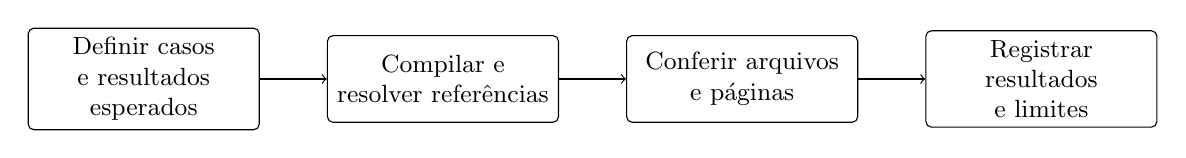
\begin{tikzpicture}[
    etapa/.style={draw, rounded corners=2pt, align=center,
      text width=2.7cm, minimum height=1.1cm, font=\small}]
    \node[etapa] (casos) at (0,0) {Definir casos\\e resultados esperados};
    \node[etapa] (compilar) at (3.8,0) {Compilar e\\resolver referências};
    \node[etapa] (conferir) at (7.6,0) {Conferir arquivos\\e páginas};
    \node[etapa] (registrar) at (11.4,0) {Registrar resultados\\e limites};
    \draw[->] (casos) -- (compilar);
    \draw[->] (compilar) -- (conferir);
    \draw[->] (conferir) -- (registrar);
  \end{tikzpicture}
  \undffonte{elaboração própria}
\end{figure}

\Needspace{7\baselineskip}
Para os complementos, foram examinados 24 destinos em cada perfil, totalizando
48 referências rotuladas. A medida utilizada foi a proporção de destinos
que apontavam para a página registrada no arquivo auxiliar, definida na
\equacaoref{correspondencia}:

\equacao[correspondencia]{C = \frac{d_{\mathrm{corretos}}}{d_{\mathrm{examinados}}}}

\noindent em que $C$ é a proporção de correspondência, $d_{\mathrm{corretos}}$
é o número de destinos coincidentes com a página prevista e
$d_{\mathrm{examinados}}$ é o total examinado. O denominador é positivo neste
corpus. A medida descreve apenas esses destinos; não é uma estimativa da
correção de todos os hyperlinks que o sistema possa gerar.

O \pseudocodigoref{destinos} sintetiza a comparação conceitual. Sua finalidade
é explicar o procedimento, sem substituir os scripts de compilação e
verificação disponíveis no repositório.

\begin{undfpseudocodigo}{CONFERIR-DESTINOS(R, P)}{destinos}{Comparação das páginas das referências rotuladas}
Entrada: rotulos R com paginas esperadas; documento PDF P
Inicio
  corretos = 0
  Para cada rotulo em R
    destino = localizar_destino(P, rotulo)
    Se pagina(destino) = pagina_esperada(rotulo)
      corretos = corretos + 1
    Fim-se
  Fim-para
  Retorne corretos / quantidade(R)
Fim
\end{undfpseudocodigo}

Nos testes bibliográficos, verificou-se se a obra original era omitida quando
usada somente na citação de citação e mantida quando citada independentemente,
antes ou depois dessa chamada. Um quarto cenário repetiu o uso indireto em
outra seção bibliográfica para verificar o isolamento da decisão. Para objetos
extensos, os critérios incluíram permanência de blocos curtos no espaço
disponível e continuação de blocos longos entre páginas.

\section{Resultados e discussão}

\subsection{Correspondência dos resultados esperados}

A \tabelaref{resultados} reúne as observações após as correções. Os 48 destinos
examinados corresponderam às páginas dos auxiliares, resultando em
$C = 48/48 = 1$. Esse valor se aplica ao conjunto finito observado e não deve
ser interpretado como probabilidade de ausência de falhas em outros documentos.

\begin{undftabela}[htb]{Síntese dos resultados da revisão local}{resultados}[elaboração própria a partir de Projeto UnDF-TeX (2026)]
  \small
  \begin{tabular}{>{\raggedright\arraybackslash}p{.25\textwidth}>{\raggedright\arraybackslash}p{.28\textwidth}>{\raggedright\arraybackslash}p{.35\textwidth}}
    \hline
    \textbf{Conjunto} & \textbf{Critério observado} & \textbf{Resultado registrado} \\
    \hline
    Modelos principais & Compilação e referências & Quatro modelos compilados com referências resolvidas \\
    Complementos & Página de destino dos rótulos & 48 correspondências em 48 destinos examinados \\
    Citação de citação & Composição da bibliografia & Quatro cenários com as listas previstas \\
    Objetos extensos & Ocupação e continuação & Blocos curtos permaneceram; objetos longos continuaram entre páginas \\
    Inclusão de PDF & Presença do conteúdo externo & Conteúdo incluído uma vez como apêndice e uma vez como anexo \\
    \hline
  \end{tabular}
\end{undftabela}

Antes das correções, a revisão reproduziu a continuação indevida da numeração
de seções no primeiro apêndice do artigo, o deslocamento de um pseudocódigo
curto apesar de haver espaço e a inclusão bibliográfica de uma obra original
usada apenas indiretamente. A inspeção também identificou títulos incorretos
em referências por nome aos complementos da monografia. As correções passaram
a distinguir as sequências e os destinos de apêndices e anexos e a separar
consulta independente de citação de citação \citeind{undf-verificacao}.

Os cenários bibliográficos mostraram que a ordem da consulta independente
não alterou a lista esperada: a obra original foi mantida tanto quando citada
antes quanto depois da chamada indireta. O cenário em outra seção bibliográfica
produziu novamente apenas a fonte consultada. Essa observação sustenta o
isolamento entre os quatro casos examinados, sem abranger todas as combinações
possíveis de comandos bibliográficos.

\subsection{Continuidade do texto e limites das evidências}

O caso de objetos extensos ocupou sete páginas. O pseudocódigo longo
atravessou as páginas 3 e 4, a tabela longa, as páginas 5 e 6, e a citação
em bloco, as páginas 6 e 7. Esses resultados mostram que os objetos escolhidos
continuaram entre páginas. Não implicam que uma figura indivisível ou uma
tabela flutuante comum possa ser dividida automaticamente. A escolha do
ambiente e das dimensões continua sendo responsabilidade de edição.

A inspeção de destinos e a revisão visual têm alcances diferentes. Um link
pode chegar à página prevista e ainda ter uma descrição pouco informativa.
Da mesma forma, um documento visualmente regular pode conter uma lista
bibliográfica incoerente. A contribuição do procedimento está em combinar
essas evidências, preservando casos pequenos que possam ser executados após
alterações nos mecanismos compartilhados.

Há limitações claras. O corpus pertence a um único projeto, e os casos foram
selecionados para investigar problemas conhecidos. Não houve amostragem
aleatória, avaliação de usabilidade, análise de desempenho ou auditoria de
acessibilidade. A execução remota da integração contínua não foi verificada
como resultado deste estudo. Também não se avaliou a correção científica de
TCCs nem o atendimento a todas as exigências normativas e institucionais.

\Needspace{12\baselineskip}
\section{Considerações finais}

A revisão forneceu evidências de consistência para os comportamentos
selecionados dos perfis de monografia e artigo: referências cruzadas dos
complementos, composição das listas bibliográficas, continuidade de objetos
e inclusão de PDF. A questão proposta foi respondida dentro desse recorte,
com correspondência dos 48 destinos e aprovação dos demais casos descritos
no registro local.

As verificações reproduzíveis ajudam a identificar regressões nos recursos
comuns e devem acompanhar a conferência visual do documento final. Recomenda-se
ampliar os casos com documentos reais, mediante autorização dos autores, e
avaliar os requisitos do curso antes da entrega.

  \printundfreferences
\end{document}
